\documentclass[12pt,a4paper]{article}

\usepackage[in, plain]{fullpage}
\usepackage{array}
\usepackage{../../../pas-math}
\usepackage{../../../moncours}


%\usepackage{pas-cours}
%-------------------------------------------------------------------------------
%          -Packages nécessaires pour écrire en Français et en UTF8-
%-------------------------------------------------------------------------------
\usepackage[utf8]{inputenc}
\usepackage[frenchb]{babel}
\usepackage[T1]{fontenc}
\usepackage{lmodern}
\usepackage{textcomp}



%-------------------------------------------------------------------------------

%-------------------------------------------------------------------------------
%                          -Outils de mise en forme-
%-------------------------------------------------------------------------------
\usepackage{hyperref}
\hypersetup{pdfstartview=XYZ}
%\usepackage{enumerate}
\usepackage{graphicx}
\usepackage{multicol}
\usepackage{tabularx}
\usepackage{multirow}


\usepackage{anysize} %%pour pouvoir mettre les marges qu'on veut
%\marginsize{2.5cm}{2.5cm}{2.5cm}{2.5cm}

\usepackage{indentfirst} %%pour que les premier paragraphes soient aussi indentés
\usepackage{verbatim}
\usepackage{enumitem}
\usepackage[usenames,dvipsnames,svgnames,table]{xcolor}

\usepackage{variations}

%-------------------------------------------------------------------------------


%-------------------------------------------------------------------------------
%                  -Nécessaires pour écrire des mathématiques-
%-------------------------------------------------------------------------------
\usepackage{amsfonts}
\usepackage{amssymb}
\usepackage{amsmath}
\usepackage{amsthm}
\usepackage{tikz}
\usepackage{xlop}
%-------------------------------------------------------------------------------



%-------------------------------------------------------------------------------


%-------------------------------------------------------------------------------
%                    - Mise en forme avancée
%-------------------------------------------------------------------------------

\usepackage{ifthen}
\usepackage{ifmtarg}


\newcommand{\ifTrue}[2]{\ifthenelse{\equal{#1}{true}}{#2}{$\qquad \qquad$}}

%-------------------------------------------------------------------------------

%-------------------------------------------------------------------------------
%                     -Mise en forme d'exercices-
%-------------------------------------------------------------------------------
%\newtheoremstyle{exostyle}
%{\topsep}% espace avant
%{\topsep}% espace apres
%{}% Police utilisee par le style de thm
%{}% Indentation (vide = aucune, \parindent = indentation paragraphe)
%{\bfseries}% Police du titre de thm
%{.}% Signe de ponctuation apres le titre du thm
%{ }% Espace apres le titre du thm (\newline = linebreak)
%{\thmname{#1}\thmnumber{ #2}\thmnote{. \normalfont{\textit{#3}}}}% composants du titre du thm : \thmname = nom du thm, \thmnumber = numéro du thm, \thmnote = sous-titre du thm

%\theoremstyle{exostyle}
%\newtheorem{exercice}{Exercice}
%
%\newenvironment{questions}{
%\begin{enumerate}[\hspace{12pt}\bfseries\itshape a.]}{\end{enumerate}
%} %mettre un 1 à la place du a si on veut des numéros au lieu de lettres pour les questions 
%-------------------------------------------------------------------------------

%-------------------------------------------------------------------------------
%                    - Mise en forme de tableaux -
%-------------------------------------------------------------------------------

\renewcommand{\arraystretch}{1.7}

\setlength{\tabcolsep}{1.2cm}

%-------------------------------------------------------------------------------



%-------------------------------------------------------------------------------
%                    - Racourcis d'écriture -
%-------------------------------------------------------------------------------

% Angles orientés (couples de vecteurs)
\newcommand{\aopp}[2]{(\vec{#1}, \vec{#2})} %Les deuc vecteurs sont positifs
\newcommand{\aopn}[2]{(\vec{#1}, -\vec{#2})} %Le second vecteur est négatif
\newcommand{\aonp}[2]{(-\vec{#1}, \vec{#2})} %Le premier vecteur est négatif
\newcommand{\aonn}[2]{(-\vec{#1}, -\vec{#2})} %Les deux vecteurs sont négatifs

%Ensembles mathématiques
\newcommand{\naturels}{\mathbb{N}} %Nombres naturels
\newcommand{\relatifs}{\mathbb{Z}} %Nombres relatifs
\newcommand{\rationnels}{\mathbb{Q}} %Nombres rationnels
\newcommand{\reels}{\mathbb{R}} %Nombres réels
\newcommand{\complexes}{\mathbb{C}} %Nombres complexes


%Intégration des parenthèses aux cosinus
\newcommand{\cosP}[1]{\cos\left(#1\right)}
\newcommand{\sinP}[1]{\sin\left(#1\right)}


%Probas stats
\newcommand{\stat}{statistique}
\newcommand{\stats}{statistiques}
%-------------------------------------------------------------------------------

%-------------------------------------------------------------------------------
%                    - Mise en page -
%-------------------------------------------------------------------------------

\newcommand{\twoCol}[1]{\begin{multicols}{2}#1\end{multicols}}


\setenumerate[1]{font=\bfseries,label=\textit{\alph*})}
\setenumerate[2]{font=\bfseries,label=\arabic*)}


%-------------------------------------------------------------------------------
%                    - Elements cours -
%-------------------------------------------------------------------------------





%\makeatletter
%\renewcommand*{\@seccntformat}[1]{\csname the#1\endcsname\hspace{0.1cm}}
%\makeatother


%\author{Olivier FINOT}
\date{}
\title{}

\graphicspath{{./img/}}

\lhead{Seq 2: Symétries}
\rhead{O. FINOT}
%
%\rfoot{Page \thepage}
\begin{document}
%\maketitle


%
%\chap[num=2, color=red]{Symétries}{Olivier FINOT, \today }
%
\begin{myobj}
	\begin{itemize}
		
		\item Construire le symétrique d’un point ou d'une figure par rapport à une droite à la main où à l’aide d’un logiciel;
		\item Construire le symétrique d’un point ou d'une figure par rapport à un point, à la main où à l’aide d’un logiciel;
		\item Utiliser les propriétés de la symétrie axiale ou centrale;
		\item Identifier des symétries dans des figures.		
	\end{itemize}
\end{myobj}

\begin{mycomp}
	\begin{itemize}
		\item \kw{Chercher (Ch2)} :  s’engager    dans    une    démarche    scientifique, observer, questionner, manipuler, expérimenter (sur une feuille de papier, avec des objets, à l’aide de logiciels), émettre des hypothèses, chercher des exemples ou des contre-exemples, simplifier ou particulariser une situation, émettre une conjecture ;
		\item \kw{Raisonner (Ra3)} :  démontrer : utiliser un raisonnement logique et des règles établies (propriétés, théorèmes, formules) pour parvenir à une conclusion ;
		\item \kw{Communiquer (Co2)} :  expliquer à l’oral ou à l’écrit (sa démarche, son raisonnement, un calcul, un protocole   de   construction   géométrique, un algorithme), comprendre les explications d’un autre et argumenter dans l’échange ; 
		
	\end{itemize}
\end{mycomp}




\begin{myobj}
	\begin{itemize}
		
		\item Construire le symétrique d’un point ou d'une figure par rapport à une droite à la main où à l’aide d’un logiciel;
		\item Construire le symétrique d’un point ou d'une figure par rapport à un point, à la main où à l’aide d’un logiciel;
		\item Utiliser les propriétés de la symétrie axiale ou centrale;
		\item Identifier des symétries dans des figures.		
	\end{itemize}
\end{myobj}

\begin{mycomp}
	\begin{itemize}
		\item \kw{Chercher (Ch2)} :  s’engager    dans    une    démarche    scientifique, observer, questionner, manipuler, expérimenter (sur une feuille de papier, avec des objets, à l’aide de logiciels), émettre des hypothèses, chercher des exemples ou des contre-exemples, simplifier ou particulariser une situation, émettre une conjecture ;
		\item \kw{Raisonner (Ra3)} :  démontrer : utiliser un raisonnement logique et des règles établies (propriétés, théorèmes, formules) pour parvenir à une conclusion ;
		\item \kw{Communiquer (Co2)} :  expliquer à l’oral ou à l’écrit (sa démarche, son raisonnement, un calcul, un protocole   de   construction   géométrique, un algorithme), comprendre les explications d’un autre et argumenter dans l’échange ; 
		
	\end{itemize}
\end{mycomp}





\begin{myexs}
	\begin{multicols}{2}
		\begin{itemize}
			\item Dans le triangle ABC ci-contre on a %$AB < AC + CB.$
			\item Un triangle de cotés 8 cm, 5 cm et 6 cm est %constructible (8 < 11)
			
			\item Le triangle $DEF$, tel que $DE = 7$ cm, $DF = 3$ cm et $FE = 4$ cm est  %plat, les points sont alignés ($4 + 3 = 7$). 
			\vspace*{1cm}
			\item Un triangle de coté 10 cm, 4 cm et 5 cm %n'est pas constructible ($10 > 4 + 5$).
		\end{itemize}
		
		
		\begin{center}
			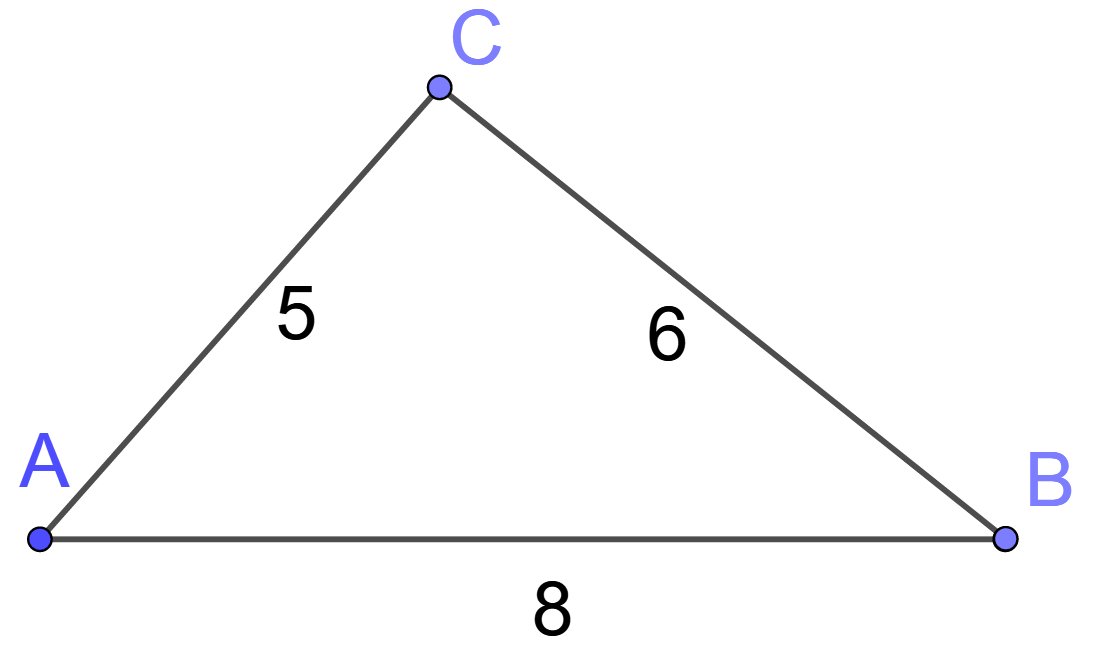
\includegraphics[scale=0.25]{triangle1}
			
			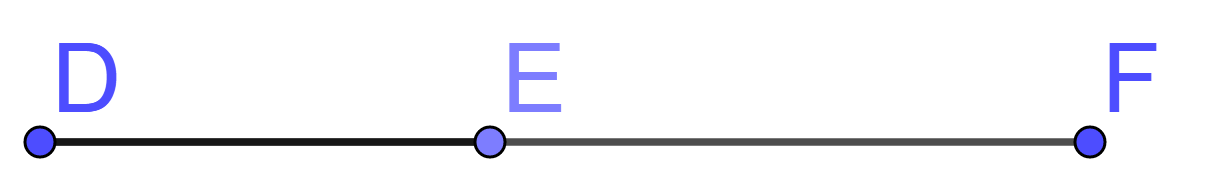
\includegraphics[scale=0.2]{triangle2}
		\end{center}
	\end{multicols}
\end{myexs}


\begin{myexs}
	\begin{multicols}{2}
		\begin{itemize}
			\item Dans le triangle ABC ci-contre on a %$AB < AC + CB.$
			\item Un triangle de cotés 8 cm, 5 cm et 6 cm est %constructible (8 < 11)
			
			\item Le triangle $DEF$, tel que $DE = 7$ cm, $DF = 3$ cm et $FE = 4$ cm est  %plat, les points sont alignés ($4 + 3 = 7$). 
			\vspace*{1cm}
			\item Un triangle de coté 10 cm, 4 cm et 5 cm %n'est pas constructible ($10 > 4 + 5$).
		\end{itemize}
		
		
		\begin{center}
			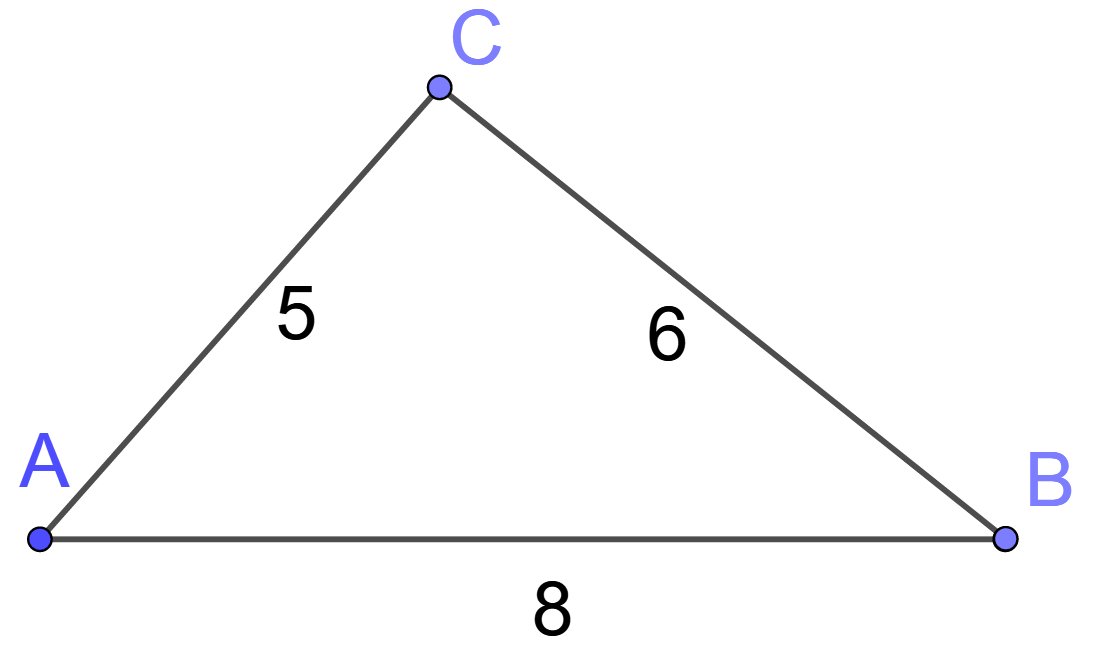
\includegraphics[scale=0.25]{triangle1}
			
			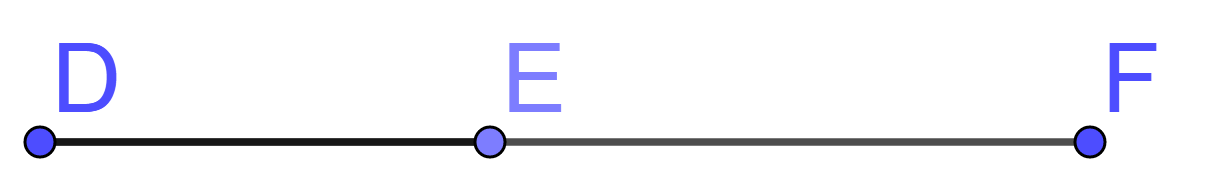
\includegraphics[scale=0.2]{triangle2}
		\end{center}
	\end{multicols}
\end{myexs}


\begin{myexs}
	\begin{multicols}{2}
		\begin{itemize}
			\item Dans le triangle ABC ci-contre on a %$AB < AC + CB.$
			\item Un triangle de cotés 8 cm, 5 cm et 6 cm est %constructible (8 < 11)
			
			\item Le triangle $DEF$, tel que $DE = 7$ cm, $DF = 3$ cm et $FE = 4$ cm est  %plat, les points sont alignés ($4 + 3 = 7$). 
			\vspace*{1cm}
			\item Un triangle de coté 10 cm, 4 cm et 5 cm %n'est pas constructible ($10 > 4 + 5$).
		\end{itemize}
		
		
		\begin{center}
			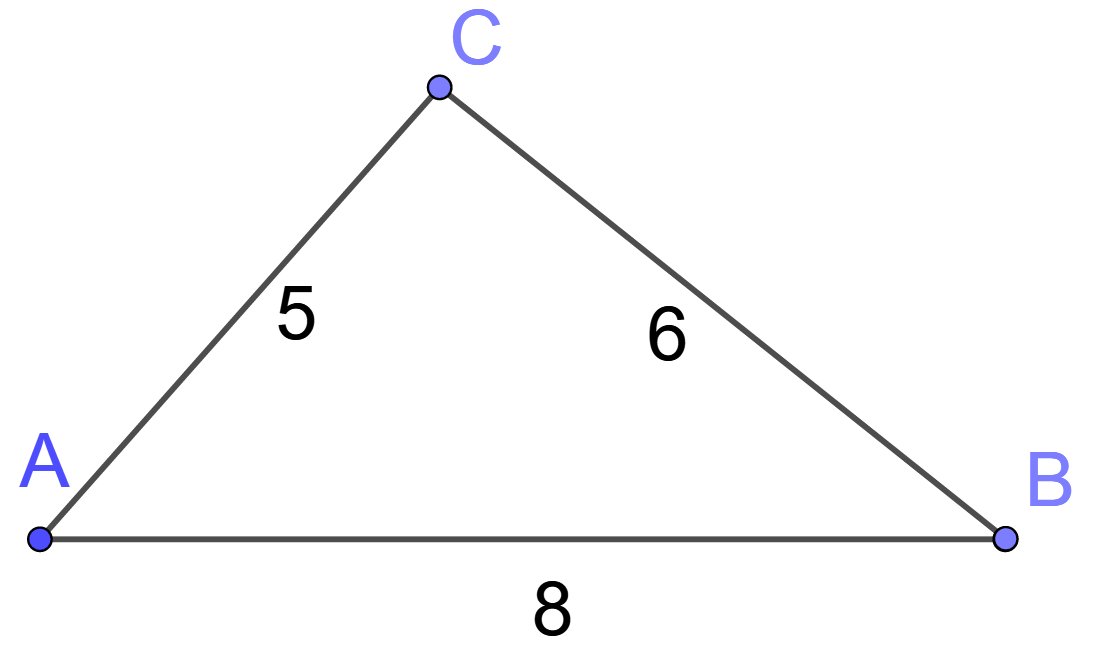
\includegraphics[scale=0.25]{triangle1}
			
			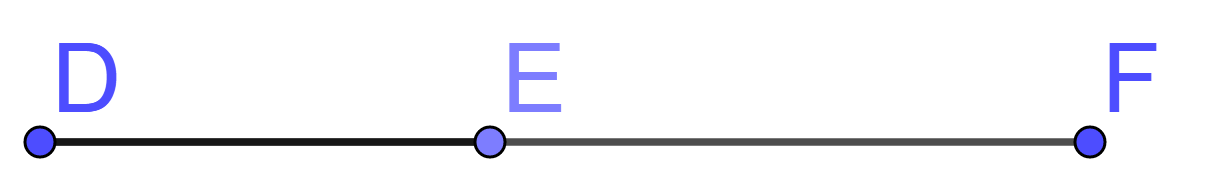
\includegraphics[scale=0.2]{triangle2}
		\end{center}
	\end{multicols}
\end{myexs}

\begin{myexs}
	\begin{multicols}{2}
		Dans la figure ci-contre :
		
		\begin{itemize}
			\item \hspace*{1cm} est la hauteur issue de \hspace*{1cm}, $H$ est le pied de cette hauteur;
			\item \hspace*{1cm} est la hauteur issue de \hspace*{1cm}, $E$ est le pied de cette hauteur;
			\item \hspace*{1cm} est la médiatrice du coté 
		\end{itemize}
		\begin{center}
			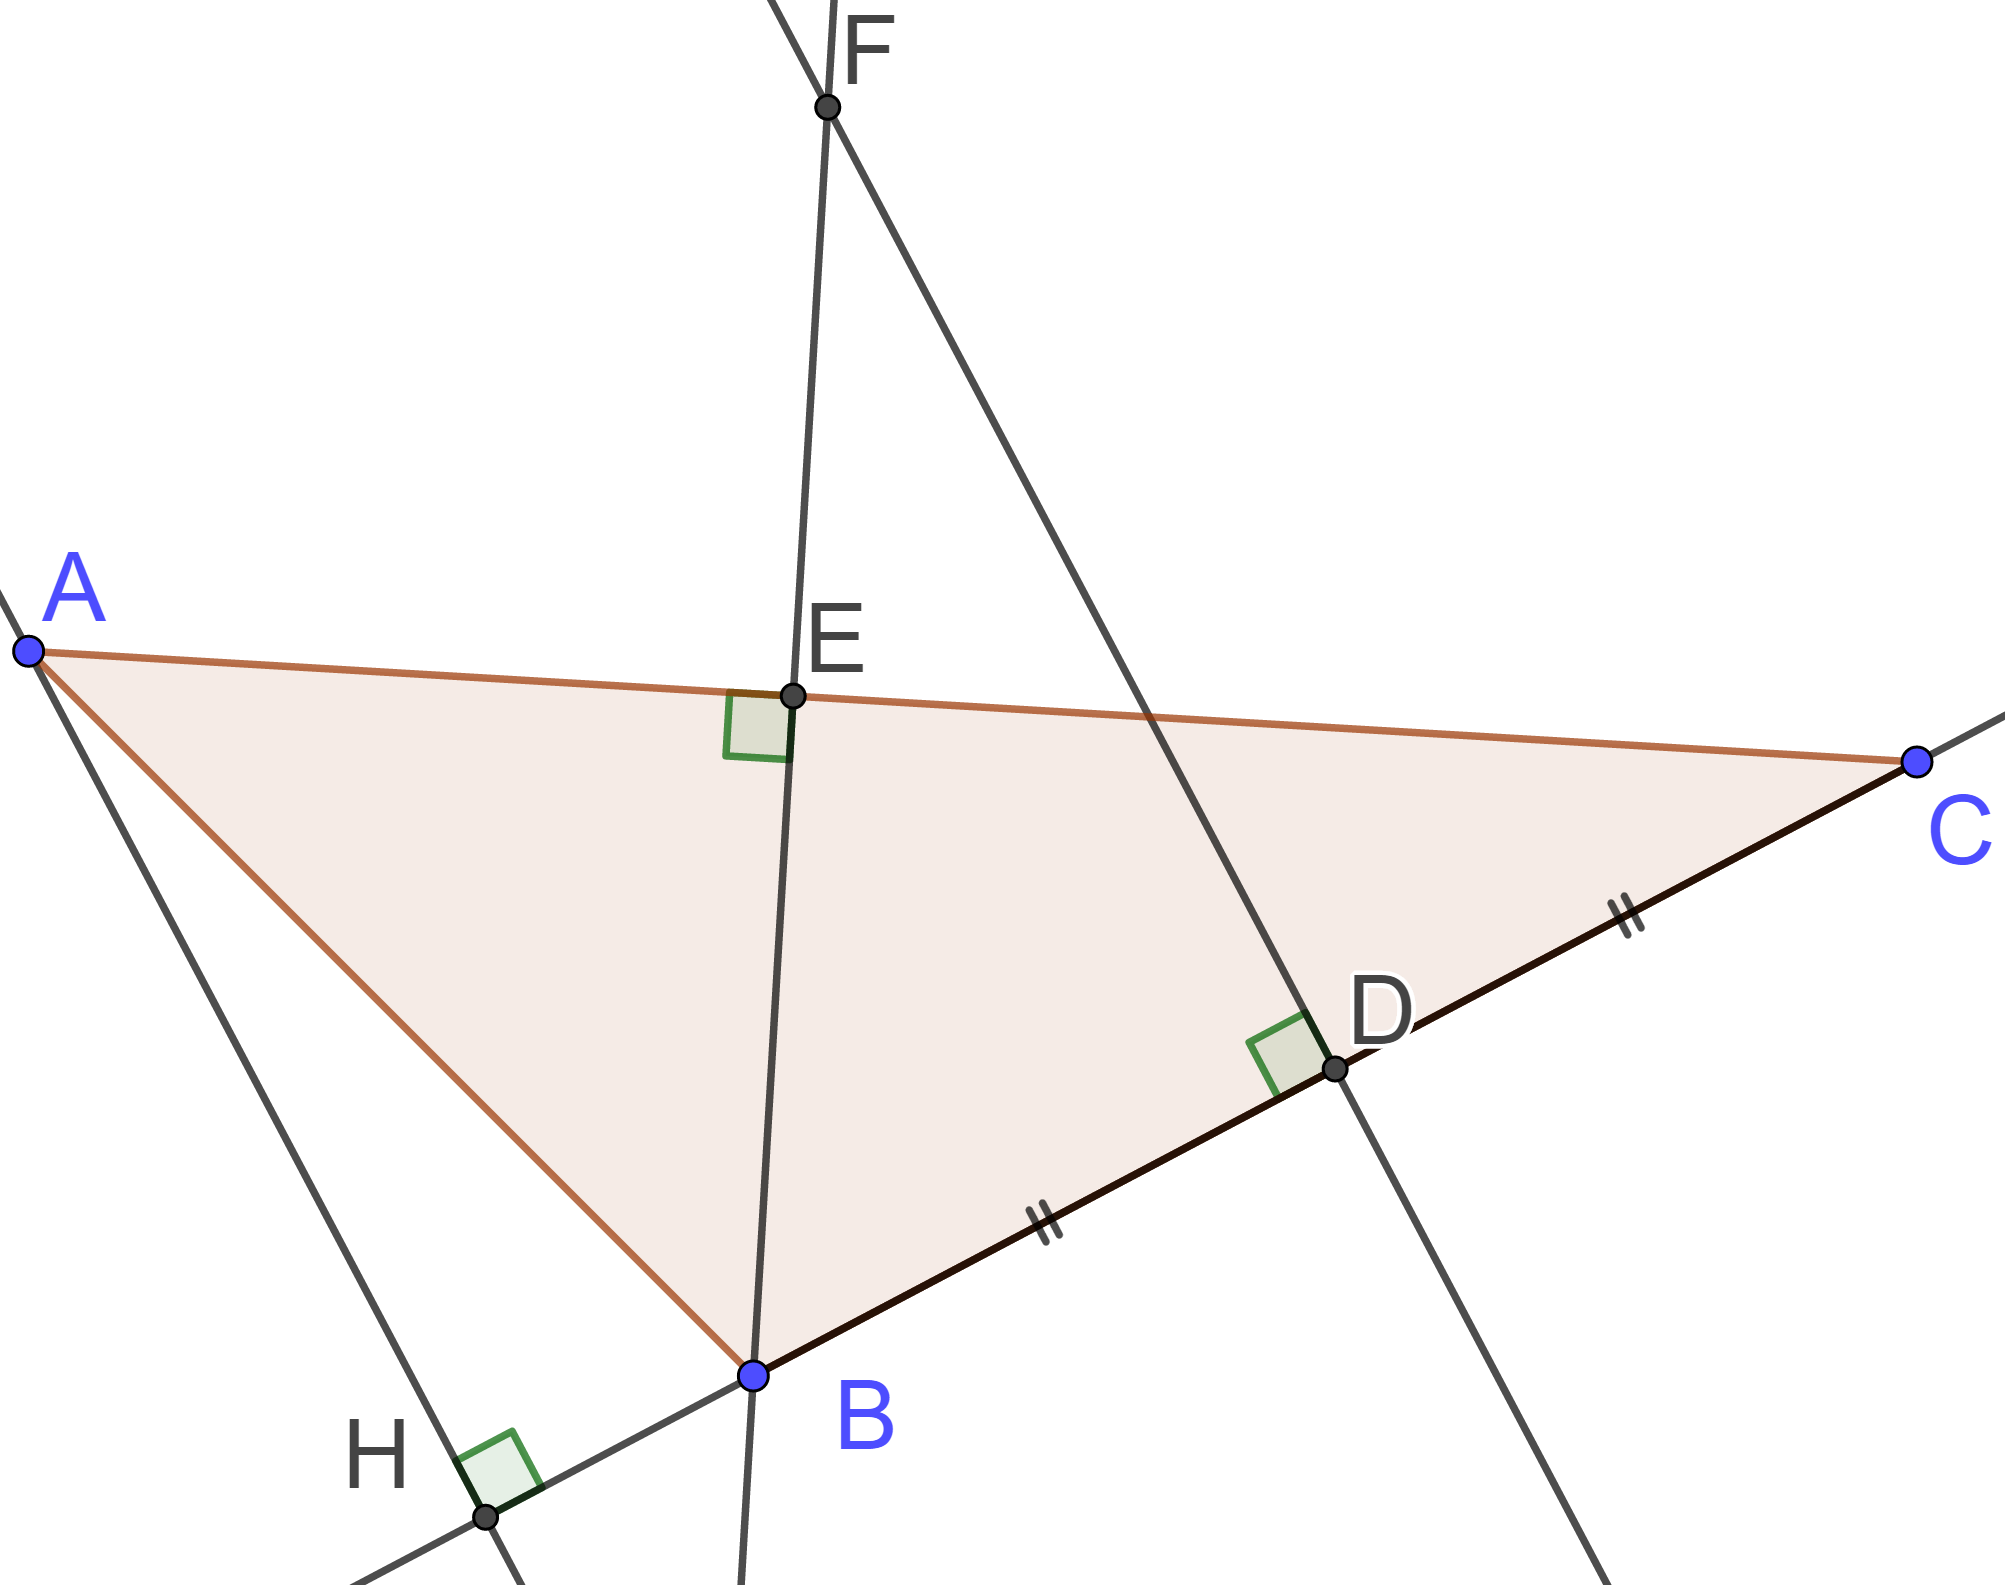
\includegraphics[scale=0.15]{droites}
		\end{center}
	\end{multicols}
\end{myexs}

\begin{myexs}
	\begin{multicols}{2}
		Dans la figure ci-contre :
		
		\begin{itemize}
			\item \hspace*{1cm} est la hauteur issue de \hspace*{1cm}, $H$ est le pied de cette hauteur;
			\item \hspace*{1cm} est la hauteur issue de \hspace*{1cm}, $E$ est le pied de cette hauteur;
			\item \hspace*{1cm} est la médiatrice du coté 
		\end{itemize}
		\begin{center}
			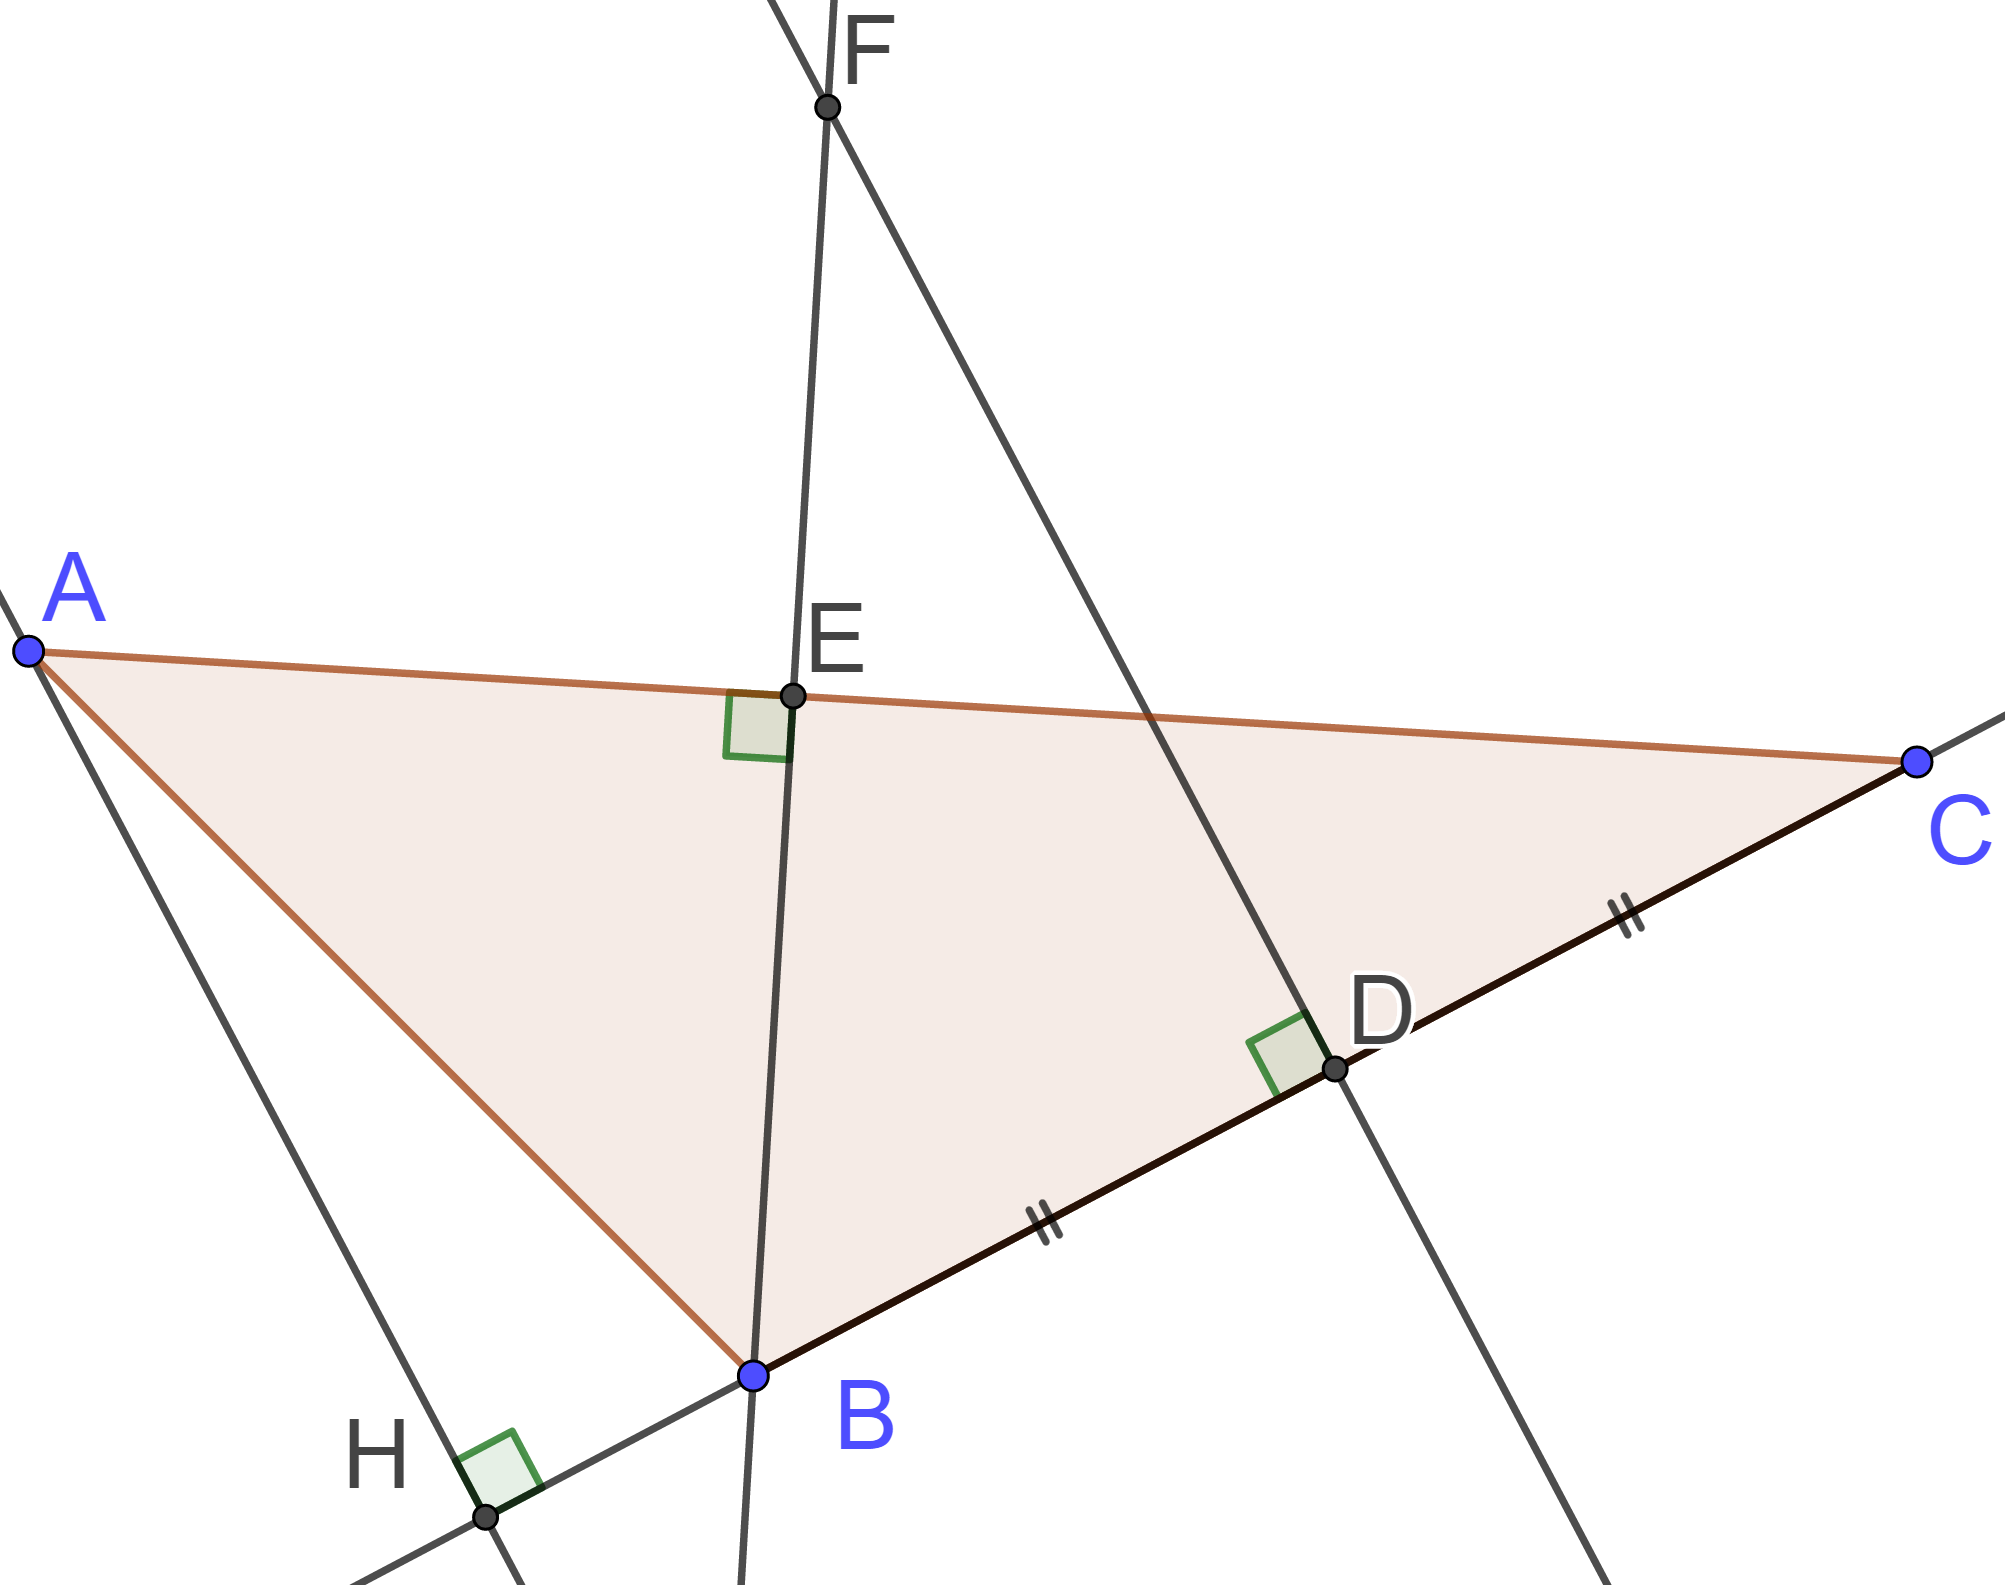
\includegraphics[scale=0.15]{droites}
		\end{center}
	\end{multicols}
\end{myexs}

\begin{myexs}
	\begin{multicols}{2}
		Dans la figure ci-contre :
		
		\begin{itemize}
			\item \hspace*{1cm} est la hauteur issue de \hspace*{1cm}, $H$ est le pied de cette hauteur;
			\item \hspace*{1cm} est la hauteur issue de \hspace*{1cm}, $E$ est le pied de cette hauteur;
			\item \hspace*{1cm} est la médiatrice du coté 
		\end{itemize}
		\begin{center}
			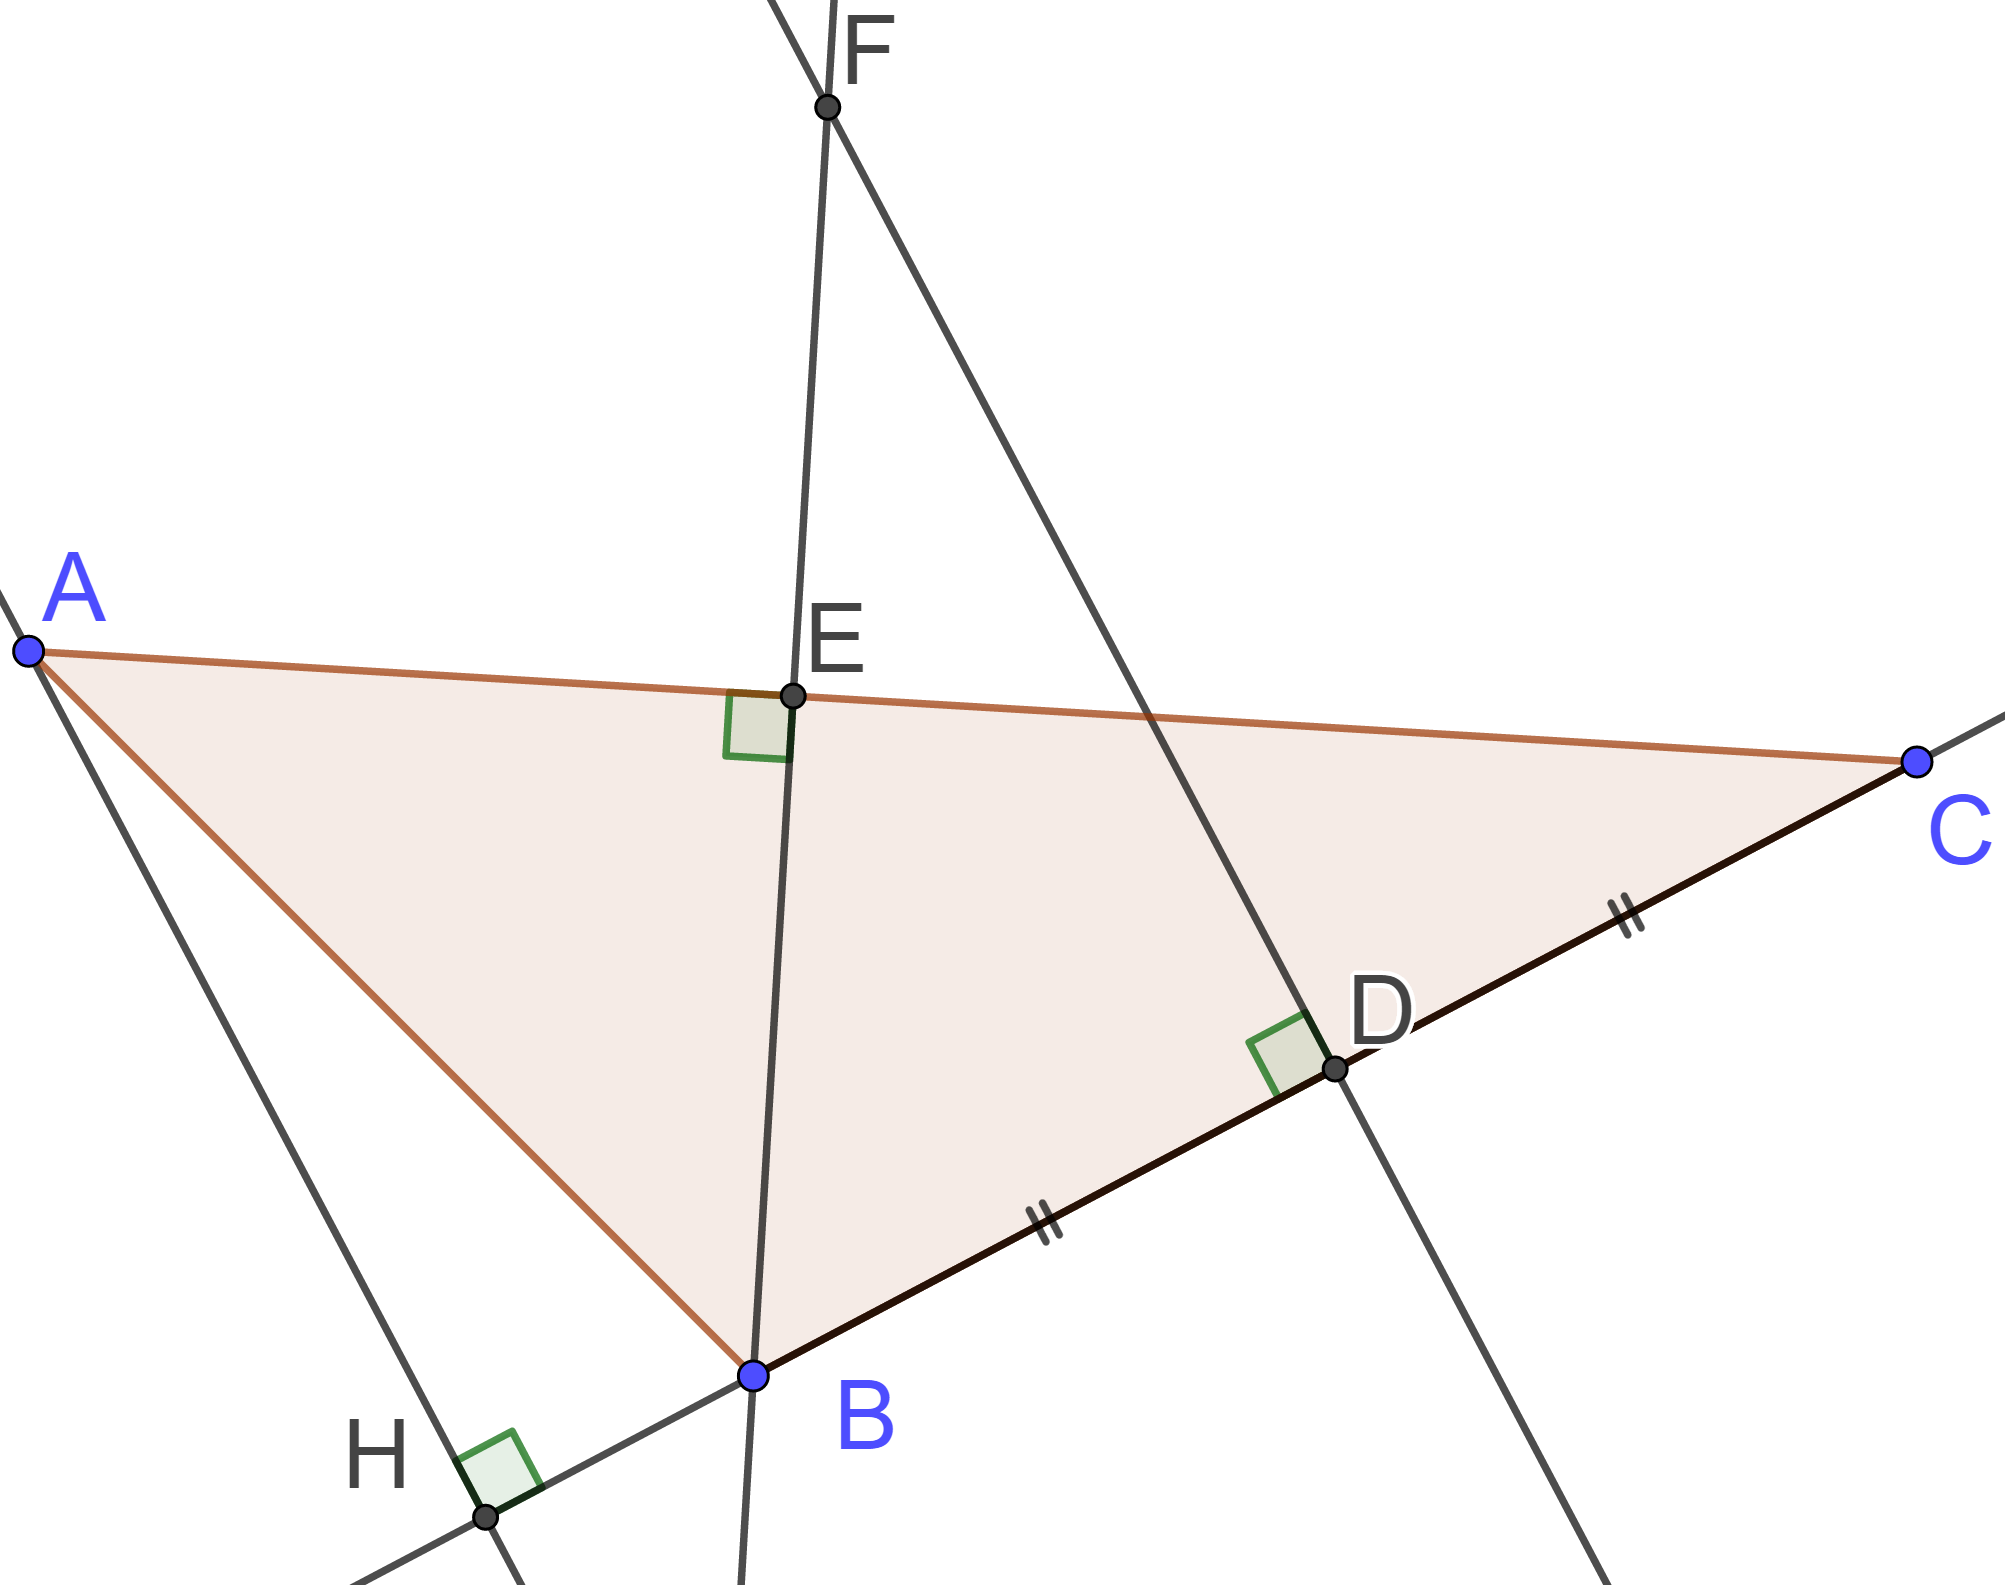
\includegraphics[scale=0.15]{droites}
		\end{center}
	\end{multicols}
\end{myexs}





\begin{myexs}
	\begin{multicols}{2}
		\vspace*{1cm}
		Dans le triangle $ABC$, on a \\ %$\hat{A} + \hat{B} + \hat{C} = 180\degree$
		\vspace*{1cm}
		
		
		Dans un triangle isocèle, les deux angles à la base sont %égaux (ici 30\degree).
		\vspace*{2.5cm}
		
		
		Dans un triangle équilatéral, tous les angles sont %égaux et mesurent 60\degree.
		
		\begin{center}	
			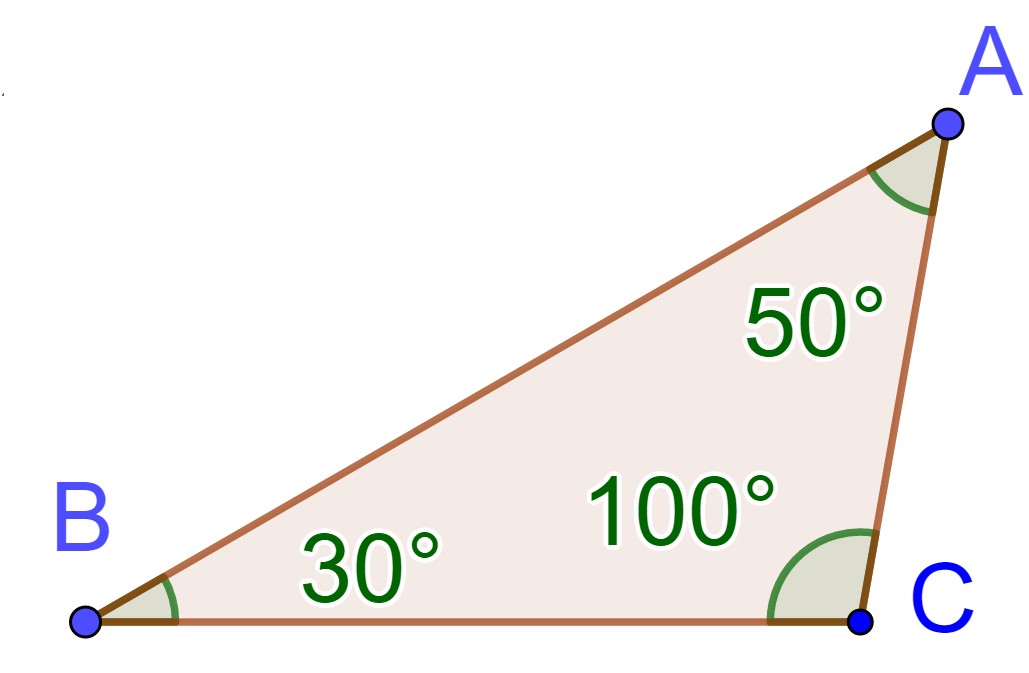
\includegraphics[scale=0.18]{quelconque}	
			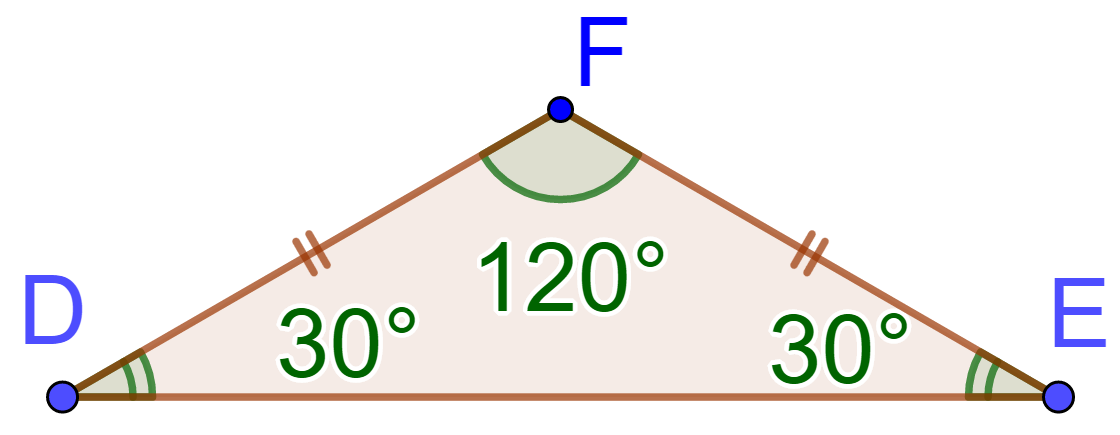
\includegraphics[scale=0.18]{isocele}	
			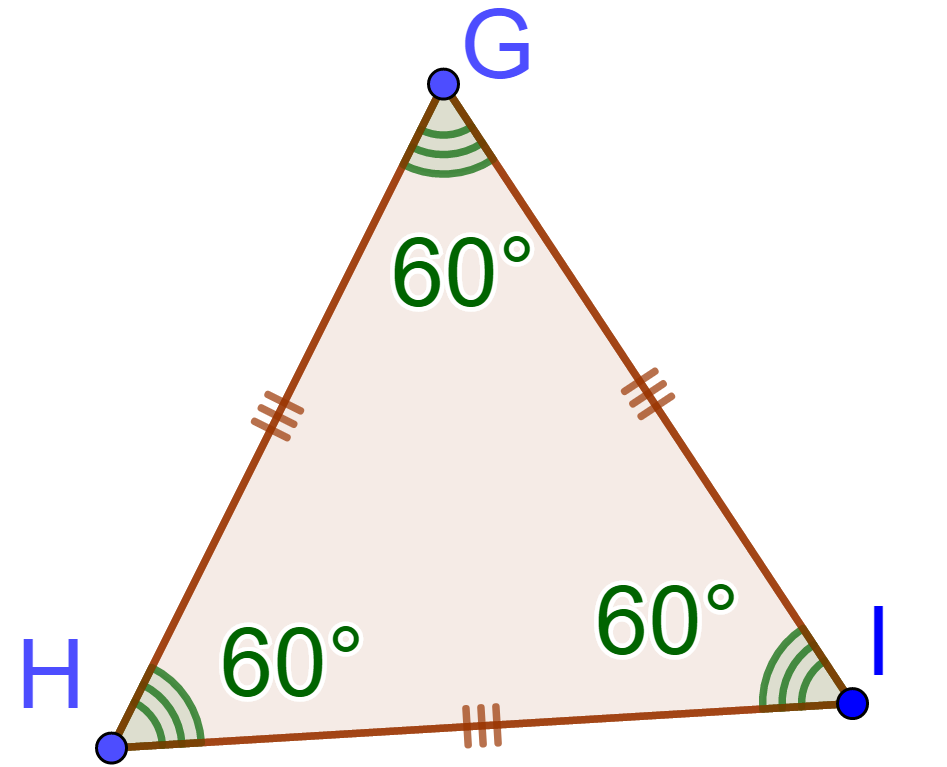
\includegraphics[scale=0.18]{equilateral}
		\end{center}
	\end{multicols}
\end{myexs}

\begin{myexs}
	\begin{multicols}{2}
		\vspace*{1cm}
		Dans le triangle $ABC$, on a \\ %$\hat{A} + \hat{B} + \hat{C} = 180\degree$
		\vspace*{1cm}
		
		
		Dans un triangle isocèle, les deux angles à la base sont %égaux (ici 30\degree).
		\vspace*{2.5cm}
		
		
		Dans un triangle équilatéral, tous les angles sont %égaux et mesurent 60\degree.
		
		\begin{center}	
			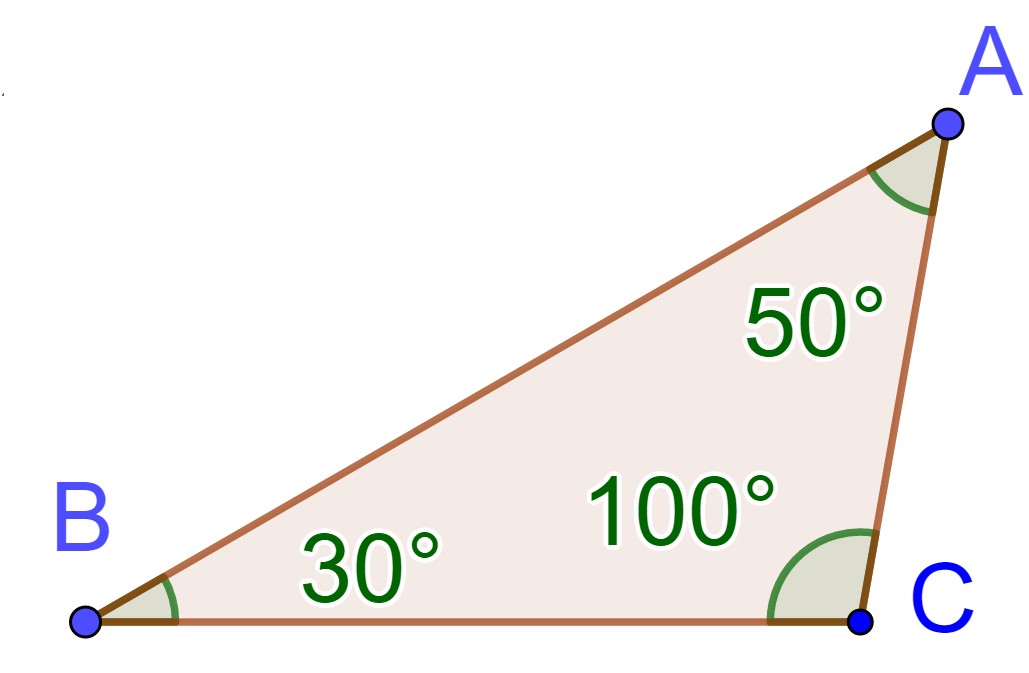
\includegraphics[scale=0.18]{quelconque}	
			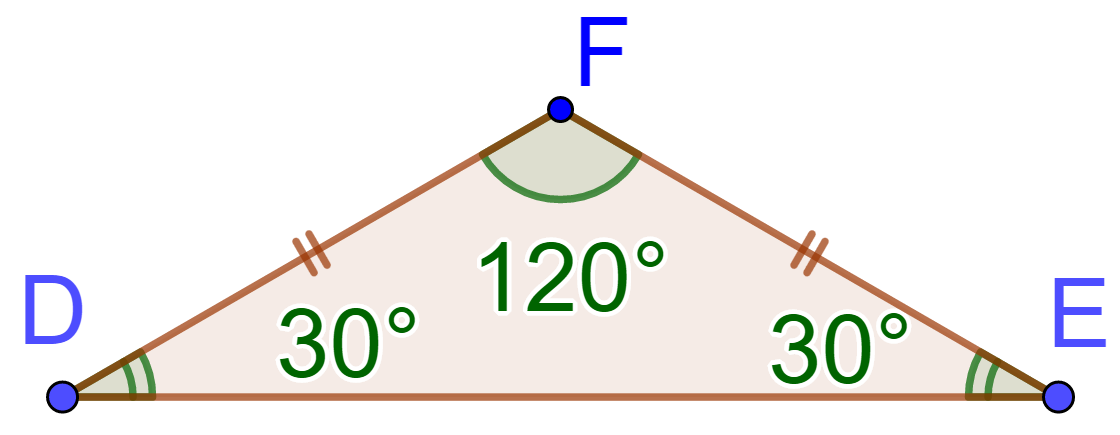
\includegraphics[scale=0.18]{isocele}	
			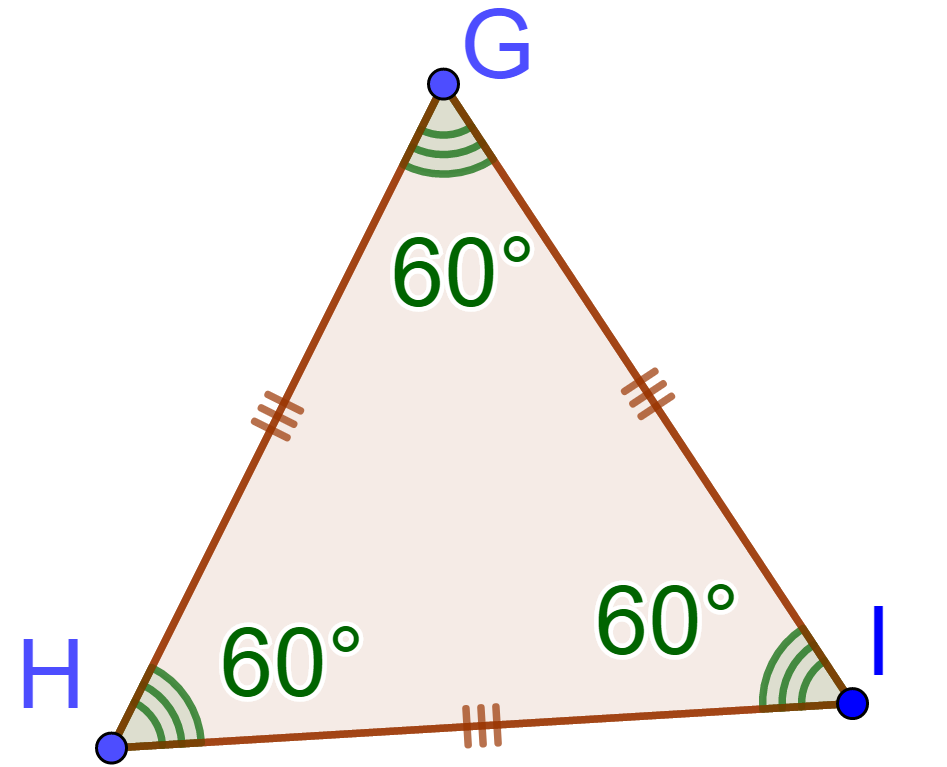
\includegraphics[scale=0.18]{equilateral}
		\end{center}
	\end{multicols}
\end{myexs}

\end{document}